\documentclass[oneside,final,12pt]{article}
\usepackage[a4paper]{geometry}
\usepackage[utf8]{inputenc}
\usepackage[T2A]{fontenc}
\usepackage[russian]{babel}
\usepackage{amssymb}
\usepackage{amsmath}
\usepackage{amsthm}
\usepackage{indentfirst}
\usepackage{parskip}
\usepackage{graphicx}
\usepackage[nottoc]{tocbibind}
\usepackage{empheq}
\usepackage{array}
% \usepackage{showframe}

\geometry{
	a4paper,onecolumn,
	left=30mm,top=20mm,right=15mm,bottom=30mm,foot=10mm,
	nohead,nomarginpar
}

\graphicspath{ {../images} }

%\setpapersize{A4}
%\setmarginsrb{3cm}{2cm}{1.5cm}{2cm}{0pt}{0mm}{0pt}{13mm}
% \sloppy
\fussy
\allowdisplaybreaks

\newtheorem{theorem}{Теорема}[section]
\newtheorem{corollary}{Следствие}[theorem]
\newtheorem{lemma}[theorem]{Лемма}

\theoremstyle{definition}
\newtheorem{definition}{Опр.}[section]

\newcommand{\R}{\mathbb{R}}
\newcommand{\vect}[1]{\boldsymbol{\overline{#1}}}
\DeclareMathOperator*{\argmax}{argmax}
\DeclareMathOperator*{\argmin}{argmin}
\DeclareMathOperator*{\grad}{grad}
\DeclareMathOperator*{\im}{Im}
\renewcommand\qedsymbol{$\blacksquare$}

\setlength{\parskip}{1.25em}
\setlength{\parindent}{0cm}
\renewcommand{\baselinestretch}{1.5}

\tolerance=1
\emergencystretch=\maxdimen
\hyphenpenalty=10000
\hbadness=10000

\begin{document}
	
	\begin{titlepage}
	
	\begin{center}
		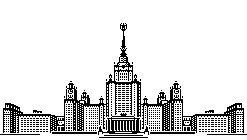
\includegraphics[scale=1.2]{msu}
		
		Московский государственный университет имени М.В.~Ломоносова\\
		Факультет вычислительной математики и кибернетики\\
		Кафедра математической физики
		
		\vspace{1.5cm}
		
		\Large{Кривоногов Роман Игоревич}
		
		\vspace{0.25cm}
		
		\textbf{\LARGE{Обратная задача для уравнения Пуассона}}
		
		\vspace{1.5cm}
		
	    \small{ВЫПУСКНАЯ КВАЛИФИКАЦИОННАЯ РАБОТА}
	\end{center}
	
	\vspace{2.5cm}
	
	\begin{flushright}
		\large{
			\textbf{Научный~руководитель:}\\
			д.ф.-м.н.,~профессор\\
			А.\,М.\,Денисов
		}
	\end{flushright}
	
	\vfill
	
	\begin{center}
		Москва, 2021
	\end{center}
	
\end{titlepage}

\pagebreak

	
    \setcounter{page}{2}
	\tableofcontents
	\pagebreak
	
	%------------------------------Section------------------------------
	\newpage
\section{Введение}



В задачах математической физики важную роль играет понятие корректности постановки задачи (или просто корректности задачи). Оно было сформулировано в 1902\,г. французским математиком Жаком Адамаром. Для описания этого понятия формализуем постановку задачи.

Пусть $u$ - известные нам данные, $z$ - неизвестные, которые предстоит определить. Предполагаем, что $u \in U$ и $z \in Z$, где $U$ и $Z$ - метрические пространства. Тогда решение задачи можно записать в виде
\[
z = R(u) \text{,}
\]
и 


Задача называется корректной по Адамару, если:

	
	%------------------------------Section------------------------------
	\section{Постановка задачи}

Рассмотрим сферу единичного радиуса с центром в начале координат $\Sigma$. Внутренность этой сферы обозначим $T$.

Пусть внутри сферы $\Sigma$ находятся $N$ точечных электрических источников с зарядами, равными единице. Координаты $i$-го источника обозначим $(x_i, y_i, z_i)$, $i = \overline{1, N}$.

Введём $3N$-вектор $\vect{v}=(x_1,y_1,z_1,x_2,y_2,z_2,...,x_N,y_N,z_N)$, определяющий координаты всех источников, и функцию
\begin{equation}
	f(x,y,z;\vect{v}) = 4\pi \sum_{i = 1}^{N} \delta(x - x_i,y - y_i,z - z_i) \text{, } (x,y,z) \in T \label{f}
\end{equation}

Пусть потенциал электрического поля на поверхности сферы равен нулю. Тогда потенциал электрического поля внутри сферы определяется задачей Дирихле для уравнения Пуассона:
\begin{empheq}[left={\empheqlbrace}]{align}
	&\Delta u(x,y,z) = - f(x,y,z;\vect{v}) \text{, } (x,y,z) \in T\text{, }\label{eqn:direct_problem_1}\\
	&u(x,y,z) = 0 \text{, } (x,y,z) \in \Sigma \text{.}\label{eqn:direct_problem_2}
\end{empheq}

Таким образом, зная положение источников $\vect{v}$ и решив задачу (\ref{eqn:direct_problem_1}), (\ref{eqn:direct_problem_2}), мы можем найти функцию $u(x,y,z)$ и вычислить нормальную производную потенциала
\[\frac{\partial u}{\partial n}(x,y,z)\text{, } (x,y,z) \in \Sigma\]
на поверхности сферы.

Сформулируем \textbf{прямую задачу}.

Задан вектор $\vect{v}$, определяющий положение источников. Требуется найти нормальную производную потенциала $\frac{\partial u}{\partial n}(x,y,z)$ на поверхности сферы.

\newpage
Сформулируем \textbf{обратную задачу 1}.

Пусть положение источников $(x_i,y_i,z_i)\text{, }i=\overline{1,N}$ неизвестно, т.е. неизвестен вектор $\vect{v}$. Требуется определить положения источников, если на поверхности сферы задана нормальная производная решения задачи (\ref{eqn:direct_problem_1}), (\ref{eqn:direct_problem_2}):
\begin{equation}
	\frac{\partial u}{\partial n}(x,y,z)=q(x,y,z) \text{, } (x,y,z) \in \Sigma \text{.} 
\end{equation}

Возможна и другая постановка обратной задачи.

\textbf{Обратная задача 2.}

Пусть положение источников $(x_i,y_i,z_i)\text{, }i=\overline{1,N}$ неизвестно, т.е. неизвестен вектор $\vect{v}$. Требуется определить положения источников, если на части $\Sigma_1$ поверхности сферы задана нормальная производная решения задачи (\ref{eqn:direct_problem_1}), (\ref{eqn:direct_problem_2}):
\begin{equation}
	\frac{\partial u}{\partial n}(x,y,z)=q(x,y,z) \text{, } (x,y,z) \in \Sigma_1 \text{.}
\end{equation}
	
	%------------------------------Section------------------------------
	\section{Редукция обратной задачи к вариационной постановке}

Найдём решение задачи (\ref{eqn:direct_problem_1}), (\ref{eqn:direct_problem_2}), используя подход, описанный в \cite[Гл.~4,~\S~4]{tikh}.

Рассмотрим сперва случай одного источника: $\vect{v} = (x_1,y_1,z_1)$. Обозначим $M_1= (x_1,y_1,z_1)$ точку, в которой он расположен; начало координат обозначим $O$ (см. рис.~\ref{fig:source_func}).

\begin{figure}[h]
	\centering
	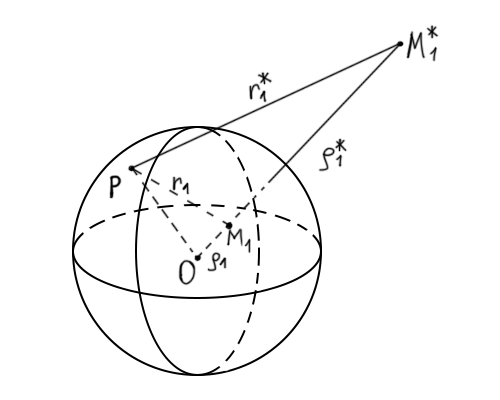
\includegraphics[scale=2]{sphere}
	\caption{Метод электростатических изображений}
	\label{fig:source_func}
\end{figure}

Воспользуемся методом функции источника: построим функцию
\begin{equation}
	G(M; M_1) = \frac{1}{ r_1} + v(M; M_1)\text{,}
\end{equation}
где $M$ --- произвольная точка из $T + \Sigma$, $r_1$ - расстояние между $M$ и $M_1$, $v$ --- некоторая гармоническая функция, непрерывная (по координатам т. $M$) в $T + \Sigma$ вместе с первыми производными, не имеющая в этом шаре особенностей и такая, что
\begin{equation}
	v\big|_\Sigma=-\frac{1}{ r_1}\text{.}
\end{equation}

Для построения воспользуемся методом электростатических изображений. Отложим на луче $OM_1$ точку $M_1^*$ такую, что
\[
OM_1 \cdot OM_1^* = 1\text{.}
\]
$M_1^*$ есть не что иное, как точка, сопряжённая с $M_1$ относительно сферы единичного радиуса с центром в начале координат.

Обозначим $\rho_1 = OM_1$ и $\rho_1^* = OM_1^*$; таким образом,
\[
\rho_1 \cdot \rho_1^* = 1\text{.}
\]

Покажем, что расстояния от всех точек $P$ поверхности сферы до $M_1$ и $M_1^*$ пропорциональны. Обозначим $r_1^*$ расстояние от $P$ до $M_1^*$.

Рассмотрим треугольники $OPM_1$ и $OPM_1^*$. Заметим, что
\[
\frac{OM_1}{OP} = \frac{OP}{OM_1^*}\text{,}
\]
и что угол при вершине $O$ - общий. Следовательно, эти треугольники подобны.

Подобие сторон
\[
\frac{OM_1}{OP} =
\frac{OP}{OM_1^*} =
\frac{PM_1}{PM_1^*}
\]
можно переписать в виде
\begin{equation}
	\frac{\rho_1}{1} =
	\frac{1}{\rho_1^*} =
	\frac{r_1}{r_1^*}\text{.}\label{proportion}
\end{equation}

Из последней пропорции следует, что
\[
r_1 = \rho r_1^*\text{,}
\]
а, значит, в качестве функции $v$ можно взять
\begin{equation}
	v(M; M_1) = - \frac{1}{ \rho_1 r_1^*}\text{.}
\end{equation}

Функция $G$ тогда принимает вид:
\begin{equation}
	G(M;M_1) =
	% \frac{1}{4 \pi}
	% \bigg(
	\frac{1}{r_1} -
	\frac{1}{\rho_1 r_1^*}
	% \bigg)
	\text{.}
\end{equation}

Полученная функция есть потенциал, создаваемый в точке $M$ единичным точечным зарядом, расположенным в точке $M_1=(x_1,y_1,z_1)$, при условии заземления поверхности сферы, т.е. решение прямой задачи (\ref{eqn:direct_problem_1}), (\ref{eqn:direct_problem_2}) для случая $\vect{v}=(x_1,y_1,z_1)$:
\begin{equation}
	u(x,y,z; \vect{v}) = 
	% \frac{1}{4 \pi}
	% \bigg(
	\frac{1}{r_1(x,y,z)} -
	\frac{1}{\rho_1 r_1^*(x,y,z)}
	% \bigg)
	\text{.}\label{eqn:potential_1}
\end{equation}

Найдём теперь нормальную производную этого потенциала на поверхности сферы. Из~(\ref{eqn:potential_1}):
\begin{equation}
	\frac{\partial u}{\partial n}
	=
	% \frac{1}{4 \pi}
	% \Bigg(
	\frac{\partial}{\partial n}
	\Big(
	\frac{1}{r_1}
	\Big)
	- \frac{1}{\rho_1}
	\frac{\partial}{\partial n}
	\Big(
	\frac{1}{r_1^*}
	\Big)
	% \Bigg)
	\text{.}\label{eqn:derivative_1}
\end{equation}

Производные по направлению внешней нормали $\mathbf{n}$ к сфере:
\begin{equation}
	\begin{aligned}
		&\frac{\partial}{\partial n}
		\Big(
		\frac{1}{r_{1}}
		\Big)
		=
		\frac{\partial}{\partial r_{1}}
		\Big(
		\frac{1}{r_{1}}
		\Big)
		\frac{\partial r_{1}}{\partial n}
		=
		-\frac{1}{r_{1}^2}
		\cos{(\widehat{\mathbf{r_{1}}, \mathbf{n}})}
		\text{,}\\[20pt]
		&\frac{\partial}{\partial n}
		\Big(
		\frac{1}{r_{1}^*}
		\Big)
		=
		\frac{\partial}{\partial r_{1}^*}
		\Big(
		\frac{1}{r_{1}^*}
		\Big)
		\frac{\partial r_{1}^*}{\partial n}
		=
		-\frac{1}{(r_{1}^*)^2}
		\cos{(\widehat{\mathbf{r_{1}^*}, \mathbf{n}})}
		\text{.}
		\label{partials}
	\end{aligned}
\end{equation}

Выразим направляющие косинусы через известные величины (см. рис. (\ref{fig:source_func})):
\begin{empheq}{align}
	&\cos{(\widehat{\mathbf{r_{1}}, \mathbf{n}})}
	=
	\frac{1 + r_{1}^2 - \rho_{1}^2}{2r_{1}}
	\text{,}\label{cos_1}\\[10pt]
	&\cos{(\widehat{\mathbf{r_{1}^*}, \mathbf{n}})}
	=
	\frac{1 + (r_{1}^*)^2 - (\rho_{1}^*)^2}{2r_{1}^*}
	\text{.}\label{cos_2}
\end{empheq}

Воспользуемся пропорциональностью (\ref{proportion}) и преобразуем (\ref{cos_2}):
\begin{equation}
	\cos{(\widehat{\mathbf{r_{1}^*}, \mathbf{n}})}
	=
	\cfrac{1 + \cfrac{r_{1}^2}{\rho_{1}^2} - \cfrac {1}{\rho_{1}^2}} {\cfrac{2 r_{1}}{\rho_{1}}}
	=
	\frac{\rho_{1}^2 + r_{1}^2 - 1}{2\rho_{1}r_{1}}
	\text{.}\label{cos_2_new}
\end{equation}

Полученные выражения для производных (\ref{partials}) и для косинусов (\ref{cos_1}), (\ref{cos_2_new}) подставим в исходное выражение (\ref{eqn:derivative_1}) для производной потенциала:
\begin{equation}
	\begin{split}
		\frac{\partial u}{\partial n}
		&=
		% \frac{1}{4 \pi}
		% \bigg[
		-\frac{1}{r_{1}^2}
		\cdot
		\frac{1 + r_{1}^2 - \rho_{1}^2}{2r_{1}}
		+
		\frac{\rho_{1}^2}{r_{1}^2}
		\cdot
		\frac{1}{\rho_{1}}
		\cdot
		\frac{\rho_{1}^2 + r_{1}^2 - 1}{2\rho_{1}r_{1}}
		% \bigg]
		=\\[10pt]
		&=
		% \frac{1}{4 \pi}
		% \cdot
		\frac{-(1 + r_{1}^2 - \rho_{1}^2) + \rho_{1}^2 + r_{1}^2 - 1}{2r_{1}^3}
		=\\[10pt]
		&=
		-
		% \frac{1}{4 \pi}
		% \cdot
		\frac{1 - \rho_{1}^2}{r_{1}^3}
		=\\[10pt]
		&=
		-
		% \frac{1}{4 \pi}
		% \cdot
		\frac{1 - x_1^2 - y_1^2 - z_1^2}
		{
			\big[
			(x - x_1)^2 + (y - y_1)^2 + (z - z_1)^2
			\big]^{\tfrac{3}{2}}}
		\text{.}\label{eqn:derivative_long_1}
	\end{split}
\end{equation}

Итак, получена нормальная производная потенциала в декартовых координатах для случая $\vect{v}=(x_1,y_1,z_1)$:
\begin{equation}
	\begin{split}
		\frac{\partial u}{\partial n}
		\Big|_\Sigma
		=
		-
		% \frac{1}{4 \pi}
		% \cdot
		\frac{1 - x_1^2 - y_1^2 - z_1^2}
		{
			\big[
			(x - x_1)^2 + (y - y_1)^2 + (z - z_1)^2
			\big]^{\tfrac{3}{2}}}
		\text{.}\label{eqn:normal_derivative_1}
	\end{split}
\end{equation}

В силу линейности задачи (\ref{eqn:direct_problem_1}), (\ref{eqn:direct_problem_2}) и оператора нормальной производной потенциал и его нормальная производная на поверхности $\Sigma$ в случае $N$ источников
\[
\vect{v}=(x_1,y_1,z_1,...,x_N,y_N,z_N)
\]
есть сумма полученных выше выражений для одного источника с соответствующей заменой индексов.

Таким образом, \textbf{решение задачи (\ref{eqn:direct_problem_1}), (\ref{eqn:direct_problem_2}) в случае $\vect{v}$ --- $3N$-мерного вектора}:
\begin{equation}
	u(x,y,z; \vect{v}) =
	% \frac{1}{4 \pi}
	\sum\limits_{i = 1}^{N}
	\bigg(
	\frac{1}{r_i(x,y,z)} -
	\frac{1}{\rho_i r_i^*(x,y,z)}
	\bigg)
	\label{eqn:potential}
\end{equation}
и его \textbf{нормальная производная на поверхности $\Sigma$}:
\begin{equation}
	\begin{split}
		\frac{\partial u}{\partial n}
		\Big|_\Sigma
		=
		-
		% \frac{1}{4 \pi}
		\sum\limits_{i = 1}^{N}
		\frac{1 - x_i^2 - y_i^2 - z_i^2}
		{
			\big[
			(x - x_i)^2 + (y - y_i)^2 + (z - z_i)^2
			\big]^{\tfrac{3}{2}}}
		\text{.}\label{eqn:normal_derivative}
	\end{split}
\end{equation}

Перейдём от вектора $\vect{v}$ к вектору $\vect{w}=\vect{w}(\vect{v}) \in \mathbb{R}^{3N}$, задающему ту же совокупность источников, но в сферических координатах. Cоответствующие преобразования координат:
\begin{equation}
	\begin{aligned}
		\rho_i
		&= 
		\sqrt{
			x_i^2 + y_i^2 + z_i^2
		}
		&\text{, }
		i=\overline{1,N}
		\text{,}
		\\[10pt]
		\phi_i
		&=
		\begin{cases}
			\begin{aligned}
				&\arctg{\frac{y_i}{x_i}}\text{, } x_i > 0\text{, } y_i > 0 \text{,}\\[5pt]
				&\arctg{\frac{y_i}{x_i}} + \pi \text{, } x_i < 0 \text{,}\\[5pt]
				&\arctg{\frac{y_i}{x_i}} + 2 \pi\text{, } x_i > 0\text{, } y_i < 0 \text{,}\\
			\end{aligned}
		\end{cases}
		&\text{, }
		i=\overline{1,N}
		\text{,}
		\\[10pt]
		\theta_i
		&=
		\arccos{
			\frac{z_i}
			{
				\sqrt{x_i^2 + y_i^2 + z_i^2}
		}}
		&\text{, }
		i=\overline{1,N}
		\text{.}
	\end{aligned}
\end{equation}

Обратные преобразования:
\begin{equation}
	\begin{aligned}
		x_i
		&=
		\rho_i \cos{\phi_i} \sin{\theta_i}
		&\text{, }
		i=\overline{1,N}
		\text{,}
		\\[10pt]
		y_i
		&=
		\rho_i \sin{\phi_i} \sin{\theta_i}
		&\text{, }
		i=\overline{1,N}
		\text{,}
		\\[10pt]
		z_i
		&=
		\rho_i \cos{\theta_i}
		&\text{, }
		i=\overline{1,N}
		\text{.}
	\end{aligned}
\end{equation}

Таким образом, ($\rho_i, \phi_i, \theta_i$) --- $i$-ый источник из $\vect{w}(\vect{v})$. Далее иногда для краткости будем писать просто~$\vect{w}$.

Введём в новых координатах обозначение для нормальной производной на поверхности сферы:
\begin{equation}
	\begin{split}
		g(\phi, \theta; \vect{w}) &=
		\frac{\partial u}{\partial n}
		\Big|_\Sigma =\\[10pt]
		&=
		-
		% \frac{1}{4 \pi}
		\sum_{i = 1}^{N} \frac{1 - \rho_i^2}
		{
			\big[
			1 + \rho_i^2 - 2\rho_i
			(cos(\phi - \phi_i)\sin\theta \sin\theta_i + \cos\theta \cos\theta_i
			)
			\big]^{\tfrac{3}{2}}}
	\end{split}
\end{equation}

Для сокращения записи введём \textbf{вспомогательную функцию}:
\begin{equation}
	K_i(\phi, \theta; \vect{w}) = 1 + \rho_i^2 - 2\rho_i(cos(\phi - \phi_i)\sin\theta \sin\theta_i + \cos\theta \cos\theta_i)\text{, }i=\overline{1,N}\text{,}
\end{equation}
тогда \textbf{нормальная производная} приобретает более компактный вид:
\begin{equation}
	\begin{split}
		g(\phi, \theta; \vect{w}) =
		\frac{\partial u}{\partial n} \Big|_\Sigma =
		-
		% \frac{1}{4 \pi}
		\sum_{i = 1}^{N}
		\frac{1 - \rho_i^2}
		{(K_i(\phi, \theta; \vect{w}))^{\tfrac{3}{2}}}
	\end{split}
\end{equation}

Сформулируем \textbf{вариационную постановку обратной задачи 1}.

Пусть на поверхности сферы известна нормальная производная $Q(\phi, \theta)$.

Требуется найти расположение источников $\vect{v}$, доставляющее минимум функции $\Phi$:
\begin{align}
	\Phi(\vect{w}(\vect{v}); Q) =
	\int\limits_{0}^{2\pi}\int\limits_{0}^{\pi}
	\big[g(\phi, \theta; \vect{w}(\vect{v})) - Q(\phi,\theta)\big]^2 
	\sin{\theta} \, d\phi \, d\theta \text{, }
	\rho_i < 1\text{, }
	i=\overline{1,N}
	\text{.}
\end{align}

Сформулируем \textbf{вариационную постановку обратной задачи 2}.

Пусть часть поверхности сферы $\Sigma_1$ определяется следующим образом:
\begin{equation}
	\Sigma_1 = \{(\rho,\phi,\theta): \rho=1\text{, }
	\phi_1 \le \phi \le \phi_2\text{, }
	\theta_1 \le \theta \le \theta_2 \}\text{.}
\end{equation}


На $\Sigma_1$ известна нормальная производная $Q(\phi, \theta)$. Требуется найти расположение источников $\vect{v}$, доставляющее минимум функции $\Phi_{\Sigma_1}$:
\begin{align}
	\Phi_{\Sigma_1}(\vect{w}(\vect{v}); Q) =
	\int\limits_{\phi_1}^{\phi_2}
	\int\limits_{\theta_1}^{\theta_2}
	\big[g(\phi, \theta; \vect{w}(\vect{v})) - Q(\phi,\theta)\big]^2 
	\sin\theta \, d\phi \, d\theta \text{, }
	\rho_i < 1\text{, }
	i=\overline{1,N}
	\text{.}
\end{align}
	
	%------------------------------Section------------------------------
	\section{Численный метод решения обратных задач}

В качестве численного метода решения обратных задач 1 и 2 в вариационной постановке предлагается использовать градиентный спуск. Минимизировать предстоит функции $\Phi$ и $\Phi_{\Sigma_1}$ соответственно.

На практике удобнее проводить минимизацию не на множестве допустимых векторов $\vect{v}$, задающих декартовы координаты источников, а на множестве соответствующих им векторов из сферических координат $\vect{w}(\vect{v})$, $\rho_i < 1$, $\overline{1,N}$. В соответствии с указанными ранее преобразованиями координат считаем $\rho_i < 1$, $\phi_i \in [0; 2\pi)$, $\theta_i \in [0; \pi]$.

Для определения направления спуска нам потребуются частные производные функций $\Phi$ и $\Phi_{\Sigma_1}$ по сферическим координатам $i$-го источника, $i = \overline{1,N}$; вычислим их для $\Phi$.

Производная по $\rho_i$:
\begin{flalign}
	% Header
	\frac{\partial \Phi}{\partial \rho_i}
	=&
	\frac{\partial}{\partial \rho_i} \Phi(\vect{w}; Q) = 
	\frac{\partial}{\partial \rho_i} \Phi(\rho_1, \phi_1, \theta_1, ..., \rho_i, \phi_i, \theta_i, ..., \rho_n, \phi_n, \theta_n; Q)
	=&&\nonumber\\[30pt]
	% First partial
	=&
	\frac{\partial}{\partial \rho_i} 
	\bigg[
	\int\limits_{0}^{2\pi}\int\limits_{0}^{\pi}
	\big[g(\phi, \theta; \vect{w}) - Q(\phi,\theta)\big]^2 
	\sin{\theta} \, d\phi \, d\theta
	\bigg]
	=&&\nonumber\\[30pt]
	% External derivative 
	=&
	2
	\cdot
	\int\limits_{0}^{2\pi}\int\limits_{0}^{\pi}
	\big[g(\phi, \theta; \vect{w}) - Q(\phi,\theta)\big]
	\cdot
	\frac{\partial}{\partial \rho_i}
	g(\phi, \theta; \vect{w})
	\cdot
	\sin{\theta} \, d\phi \, d\theta
	=&&\nonumber\\[30pt]
	% Internal derivative
	=&
	2
	\cdot
	\int\limits_{0}^{2\pi}\int\limits_{0}^{\pi}
	\big[g(\phi, \theta; \vect{w}) - Q(\phi,\theta)\big]
	\cdot&&\nonumber\\[10pt]
	\cdot&
	\bigg[
	(-1)
	\cdot
	\frac{-2\rho_i K_i(\phi, \theta; \vect{w})^{\tfrac{3}{2}}
		-
		(1 - \rho_i^2)
		\cdot
		\tfrac{3}{2}
		K_i(\phi, \theta; \vect{w})^{\tfrac{1}{2}}
		\cdot
		\frac{\partial}{\partial \rho_i}
		K_i(\phi, \theta; \vect{w})
	}
	{K_i(\phi, \theta; \vect{w})^3}
	\bigg]
	\cdot
	\sin{\theta} \, d\phi \, d\theta
	=&&\nonumber\\[30pt]
	% Reduction
	=&
	\int\limits_{0}^{2\pi}\int\limits_{0}^{\pi}
	\big[g(\phi, \theta; \vect{w}) - Q(\phi,\theta)\big]
	\cdot&&\nonumber\\[10pt]
	\cdot&
	\frac{4 \rho_i K_i(\phi, \theta; \vect{w})
		+ 3 (1 - \rho_i^2)
		\big[
		2\rho_i - 2
		(\cos(\phi - \phi_i)\sin\theta\sin\theta_i + \cos\theta\cos\theta_i)
		\big]}
	{K_i(\phi, \theta; \vect{w})^{\tfrac{5}{2}}}
	\cdot
	\sin{\theta} \, d\phi \, d\theta
	=&&\nonumber\\[30pt]
	% Final
	=&
	\int\limits_{0}^{2\pi}\int\limits_{0}^{\pi}
	\big[
	g(\phi, \theta; \vect{w})
	- Q(\phi,\theta)
	\big]
	\cdot&&\nonumber\\[10pt]
	\cdot&
	\bigg[
	\frac{4\rho_i}{K_i(\phi, \theta; \vect{w})^{\tfrac{3}{2}}}
	+
	6 \cdot
	\frac{(1 - \rho_i^2)
		\big[
		\rho_i - (\cos(\phi - \phi_i)\sin\theta\sin\theta_i + \cos\theta\cos\theta_i)
		\big]}
	{K_i(\phi, \theta; \vect{w})^{\tfrac{5}{2}}}
	\bigg]
	\cdot&&\nonumber\\[10pt]
	\cdot&
	\sin{\theta} \, d\phi \, d\theta
	\text{.}&&
\end{flalign}

Производная по $\phi_i$:
\begin{flalign}
	% Header
	\frac{\partial \Phi}{\partial \phi_i}
	=&
	\frac{\partial}{\partial \phi_i} \Phi(\vect{w}; Q) = 
	\frac{\partial}{\partial \phi_i} \Phi(\rho_1, \phi_1, \theta_1, ..., \rho_i, \phi_i, \theta_i, ..., \rho_n, \phi_n, \theta_n; Q)
	=&&\nonumber\\[30pt]
	% First partial
	=&
	\frac{\partial}{\partial \phi_i} 
	\bigg[
	\int\limits_{0}^{2\pi}\int\limits_{0}^{\pi}
	\big[g(\phi, \theta; \vect{w}) - Q(\phi,\theta)\big]^2 
	\sin{\theta} \, d\phi \, d\theta
	\bigg]
	=&&\nonumber\\[30pt]
	% External derivative 
	=&
	2 \cdot
	\int\limits_{0}^{2\pi}\int\limits_{0}^{\pi}
	\big[g(\phi, \theta; \vect{w}) - Q(\phi,\theta)\big]
	\cdot
	\frac{\partial}{\partial \phi_i}
	g(\phi, \theta; \vect{w})
	\sin{\theta} \, d\phi \, d\theta
	=&&\nonumber\\[30pt]
	% Internal derivative
	=&
	2 \cdot
	\int\limits_{0}^{2\pi}\int\limits_{0}^{\pi}
	\big[g(\phi, \theta; \vect{w}) - Q(\phi,\theta)\big]
	\cdot&&\nonumber\\[10pt]
	\cdot&
	\bigg[
	(-1)
	\cdot
	\frac{
		-
		(1 - \rho_i^2)
		\cdot
		\tfrac{3}{2}
		K_i(\phi, \theta; \vect{w})^{\tfrac{1}{2}}
		\cdot
		\frac{\partial}{\partial \phi_i}
		K_i(\phi, \theta; \vect{w})
	}
	{K_i(\phi, \theta; \vect{w})^3}
	\bigg]
	\cdot
	\sin{\theta} \, d\phi \, d\theta
	=&&\nonumber\\[30pt]
	% Reduction
	=&
	\int\limits_{0}^{2\pi}\int\limits_{0}^{\pi}
	\big[g(\phi, \theta; \vect{w}) - Q(\phi,\theta)\big]
	\cdot&&\nonumber\\[10pt]
	\cdot&
	\frac{3 (1 - \rho_i^2)( - 2 \rho_i
		\sin(\phi - \phi_i)\sin\theta\sin\theta_i
		)}
	{K_i(\phi, \theta; \vect{w})^{\tfrac{5}{2}}}
	\cdot
	\sin{\theta} \, d\phi \, d\theta
	=&&\nonumber\\[30pt]
	% Final
	=&
	-6
	\int\limits_{0}^{2\pi}\int\limits_{0}^{\pi}
	\big[
	g(\phi, \theta; \vect{w})
	- Q(\phi,\theta)
	\big]
	\cdot
	\bigg[
	\frac{(1 - \rho_i^2)\rho_i\sin(\phi - \phi_i)\sin{\theta}\sin{\theta_i}}
	{K_i(\phi, \theta; \vect{w})^{\tfrac{5}{2}}}
	\bigg]
	\cdot
	\sin{\theta} \, d\phi \, d\theta
	\text{.}&&
\end{flalign}

Производная по $\theta_i$:
\begin{flalign}
	% Header
	\frac{\partial \Phi}{\partial \theta_i}
	=&
	\frac{\partial}{\partial \theta_i} \Phi(\vect{w}; Q) = 
	\frac{\partial}{\partial \theta_i} \Phi(\rho_1, \phi_1, \theta_1, ..., \rho_i, \phi_i, \theta_i, ..., \rho_n, \phi_n, \theta_n; Q)
	=&&\nonumber\\[30pt]
	% First partial
	=&
	\frac{\partial}{\partial \theta_i} 
	\bigg[
	\int\limits_{0}^{2\pi}\int\limits_{0}^{\pi}
	\big[g(\phi, \theta; \vect{w}) - Q(\phi,\theta)\big]^2 
	\sin\theta \, d\phi \, d\theta
	\bigg]
	=&&\nonumber\\[30pt]
	% External derivative 
	=&
	2 \cdot
	\int\limits_{0}^{2\pi}\int\limits_{0}^{\pi}
	\big[g(\phi, \theta; \vect{w}) - Q(\phi,\theta)\big]
	\cdot
	\frac{\partial}{\partial \theta_i}
	g(\phi, \theta; \vect{w})
	\sin{\theta} \, d\phi \, d\theta
	=&&\nonumber\\[30pt]
	% Internal derivative
	=&
	2 \cdot
	\int\limits_{0}^{2\pi}\int\limits_{0}^{\pi}
	\big[g(\phi, \theta; \vect{w}) - Q(\phi,\theta)\big]
	\cdot&&\nonumber\\[10pt]
	\cdot&
	\bigg[
	(-1)
	\cdot
	\frac{
		-
		(1 - \rho_i^2)
		\cdot
		\tfrac{3}{2}
		K_i(\phi, \theta; \vect{w})^{\tfrac{1}{2}}
		\cdot
		\frac{\partial}{\partial \theta_i}
		K_i(\phi, \theta; \vect{w})
	}
	{K_i(\phi, \theta; \vect{w})^3}
	\bigg]
	\cdot
	\sin\theta \, d\phi \, d\theta
	=&&\nonumber\\[30pt]
	% Reduction
	=&
	\int\limits_{0}^{2\pi}\int\limits_{0}^{\pi}
	\big[g(\phi, \theta; \vect{w}) - Q(\phi,\theta)\big]
	\cdot&&\nonumber\\[10pt]
	\cdot&
	\frac{3 (1 - \rho_i^2)
		\big[
		-2\rho_i
		(\cos(\phi - \phi_i)\sin\theta\cos\theta_i
		-
		\cos\theta\sin\theta_i)
		\big]}
	{K_i(\phi, \theta; \vect{w})^{\tfrac{5}{2}}}
	\cdot
	\sin{\theta} \, d\phi \, d\theta
	=&&\nonumber\\[30pt]
	% Final
	=&
	-6
	\int\limits_{0}^{2\pi}\int\limits_{0}^{\pi}
	\big[
	g(\phi, \theta; \vect{w})
	- Q(\phi,\theta)
	\big]
	\cdot&&\nonumber\\[10pt]
	\cdot&
	\bigg[
	\frac{(1 - \rho_i^2)
		\rho_i(\cos(\phi - \phi_i)\sin\theta\cos\theta_i - \cos\theta\sin\theta_i)}
	{K_i(\phi, \theta; \vect{w})^{\tfrac{5}{2}}}
	\bigg]
	\cdot
	\sin{\theta} \, d\phi \, d\theta
	\text{.}&&
\end{flalign}

\newpage
\textbf{Итоговые частные производные функции $\Phi$:}
\begin{flalign}
	% Header
	\frac{\partial \Phi}{\partial \rho_i}
	=&
	\int\limits_{0}^{2\pi}\int\limits_{0}^{\pi}
	\big[
	g(\phi, \theta; \vect{w})
	- Q(\phi,\theta)
	\big] \cdot
	\bigg[
	\frac{4\rho_i}{K_i(\phi, \theta; \vect{w})^{\tfrac{3}{2}}}
	+&&\nonumber\\[10pt]
	+&
	6 \cdot
	\frac{(1 - \rho_i^2)
		\big[
		\rho_i - (\cos(\phi - \phi_i)\sin\theta\sin\theta_i + \cos\theta\cos\theta_i)
		\big]}
	{K_i(\phi, \theta; \vect{w})^{\tfrac{5}{2}}}
	\bigg]
	\cdot
	\sin{\theta} \, d\phi \, d\theta
	\text{,}&&
\end{flalign}
\begin{flalign}
	% Header
	\frac{\partial \Phi}{\partial \phi_i}
	=&
	-6
	\int\limits_{0}^{2\pi}\int\limits_{0}^{\pi}
	\big[
	g(\phi, \theta; \vect{w})
	- Q(\phi,\theta)
	\big]
	\cdot&&\nonumber\\[10pt]
	\cdot&
	\bigg[
	\frac{(1 - \rho_i^2)\rho_i\sin(\phi - \phi_i)\sin{\theta}\sin{\theta_i}}
	{K_i(\phi, \theta; \vect{w})^{\tfrac{5}{2}}}
	\bigg]
	\cdot
	\sin{\theta} \, d\phi \, d\theta
	\text{,}&&
\end{flalign}
\begin{flalign}
	% Header
	\frac{\partial \Phi}{\partial \theta_i}
	=&
	-6
	\int\limits_{0}^{2\pi}\int\limits_{0}^{\pi}
	\big[
	g(\phi, \theta; \vect{w})
	- Q(\phi,\theta)
	\big]
	\cdot&&\nonumber\\[10pt]
	\cdot&
	\bigg[
	\frac{(1 - \rho_i^2)
		\rho_i(\cos(\phi - \phi_i)\sin\theta\cos\theta_i - \cos\theta\sin\theta_i)}
	{K_i(\phi, \theta; \vect{w})^{\tfrac{5}{2}}}
	\bigg]
	\cdot
	\sin{\theta} \, d\phi \, d\theta
	\text{.}&&
\end{flalign}

Частные производные функции $\Phi_{\Sigma_1}$ вычисляются аналогично, поэтому приведём лишь итоговые формулы:
\begin{flalign}
	% Header
	\frac{\partial \Phi_{\Sigma_1}}{\partial \rho_i}
	=&
	\int\limits_{\phi_1}^{\phi_2}\int\limits_{\theta_1}^{\theta_2}
	\big[
	g(\phi, \theta; \vect{w})
	- Q(\phi,\theta)
	\big] \cdot
	\bigg[
	\frac{4\rho_i}{K_i(\phi, \theta; \vect{w})^{\tfrac{3}{2}}}
	+&&\nonumber\\[10pt]
	+&
	6 \cdot
	\frac{(1 - \rho_i^2)
		\big[
		\rho_i - (\cos(\phi - \phi_i)\sin\theta\sin\theta_i + \cos\theta\cos\theta_i)
		\big]}
	{K_i(\phi, \theta; \vect{w})^{\tfrac{5}{2}}}
	\bigg]
	\cdot
	\sin{\theta} \, d\phi \, d\theta
	\text{,}&&
\end{flalign}
\begin{flalign}
	% Header
	\frac{\partial \Phi_{\Sigma_1}}{\partial \phi_i}
	=&
	-6
	\int\limits_{\phi_1}^{\phi_2}\int\limits_{\theta_1}^{\theta_2}
	\big[
	g(\phi, \theta; \vect{w})
	- Q(\phi,\theta)
	\big]
	\cdot&&\nonumber\\[10pt]
	\cdot&
	\bigg[
	\frac{(1 - \rho_i^2)\rho_i\sin(\phi - \phi_i)\sin{\theta}\sin{\theta_i}}
	{K_i(\phi, \theta; \vect{w})^{\tfrac{5}{2}}}
	\bigg]
	\cdot
	\sin{\theta} \, d\phi \, d\theta
	\text{,}&&
\end{flalign}
\begin{flalign}
	% Header
	\frac{\partial \Phi_{\Sigma_1}}{\partial \theta_i}
	=&
	-6
	\int\limits_{\phi_1}^{\phi_2}\int\limits_{\theta_1}^{\theta_2}
	\big[
	g(\phi, \theta; \vect{w})
	- Q(\phi,\theta)
	\big]
	\cdot&&\nonumber\\[10pt]
	\cdot&
	\bigg[
	\frac{(1 - \rho_i^2)
		\rho_i(\cos(\phi - \phi_i)\sin\theta\cos\theta_i - \cos\theta\sin\theta_i)}
	{K_i(\phi, \theta; \vect{w})^{\tfrac{5}{2}}}
	\bigg]
	\cdot
	\sin{\theta} \, d\phi \, d\theta
	\text{.}&&
\end{flalign}

\emph{Опишем градиентный метод} решения задачи минимизации функции. За основу берётся метод из \cite{vasil'yev} с небольшими изменениями. Изложение будем вести для функции $\Phi$, для $\Phi_{\Sigma_1}$ рассуждения аналогичны приведённым ниже.

В качестве начального приближения для небольшого $N$ ($N \le 7$) будем рассматривать подмножества без повторов из $N$ элементов следующего множества точек (заданных в декартовых координатах):
\[
\lbrace
(0, 0, 0)\text{, }
(0.5, 0, 0)\text{, }
(-0.5, 0, 0)\text{, }
(0, 0.5, 0)\text{, }
(0, -0.5, 0)\text{, }
(0, 0, 0.5)\text{, }
(0, 0, -0.5)
\rbrace
\text{.}
\]

Путём перебора всевозможных сочетаний по $N$ точек из приведённых семи выберем начальное приближение, на котором значение функции $\Phi$ минимально. Координаты этих точек образуют вектор $\vect{v}_1$. Предложенный метод позволяет найти близкое начальное приближение и в то же время помогает избежать "слипания" источников друг с другом на начальном этапе.

Градиентный спуск будем осуществлять следующим образом: вычислим для очередного (с номером $k$) приближения координат $\vect{v}_k$, $k=1,2,...$ градиент $\nabla \Phi(\vect{w}(\vect{v}_k))$. Получим $N + 1$ возможных направлений движения:
\begin{align}
    \vect{s}_{k0} =& \nabla \Phi(\vect{w}(\vect{v}_k))
    =
    \nabla \Phi(\vect{w}_k)
    \text{,}\\
    \vect{s}_{ki} =& (0,0,0,...,
    \frac{\partial}{\partial \rho_i} \Phi(\vect{w}_k),
    \frac{\partial}{\partial \phi_i} \Phi(\vect{w}_k),
    \frac{\partial}{\partial \theta_i} \Phi(\vect{w}_k),
    ...,0,0,0)
    \text{, }
    i = \overline{1,N}
    \text{.}
\end{align}

Начинаем с величины шага $\alpha_k^1 = 1$. Выбираем направление, в котором следует делать шаг данной величины:
\begin{equation}
    \vect{s}_k^1 = \argmin_{\vect{s}_{ki}} \Phi(\vect{w}_k - \alpha_k^1 \vect{s}_{ki}) \text{.}
\end{equation}

Далее для полученного направления $\vect{s}_k^1$ проверяется, выполнено ли
\begin{align}
    &\vect{w}_k - \alpha_k^1 \vect{s}_k^1 \in T \text{,}\\
    &\Phi(\vect{w}_k - \alpha_k^1 \vect{s}_k^1) < \Phi(\vect{w}_k) \text{.}
\end{align}
Если это условие выполнено, то полагаем $\vect{w}_{k+1} = \vect{w}_{k} - \alpha_k^1 \vect{s}_k^1$ и переходим к $k + 1$ итерации. В противном случае уменьшаем величину шага: $\alpha_k^{2} = \frac{\alpha_k^1}{2}$ или, в общем случае,
\begin{equation}
    \alpha_k^{j} = \frac{\alpha_k^{j - 1}}{2} \text{, } j = 2,3,... \text{,}
\end{equation}
 и повторяем описанный выше процесс выбора направления и его проверки:
\begin{align}
    &\vect{s}_k^j = \argmin_{\vect{s}_{ki}} \Phi(\vect{w}_k - \alpha_k^j \vect{s}_{ki}) \text{,}\\
    &\vect{w}_k - \alpha_k^j \vect{s}_k^j \in T \text{,}\\
    &\Phi(\vect{w}_k - \alpha_k^j \vect{s}_k^j) < \Phi(\vect{w}_k) \text{.}
\end{align}

Когда подходящие $\vect{s}_k^j$ и $\alpha_k^j$ найдены (для достаточно малой окрестности точки $\vect{v}_k$ это гарантировано в силу дифференцируемости), полагаем $\vect{s}_k = \vect{s}_k^j$ и $\alpha_k = \alpha_k^j$ и
\begin{equation}
\vect{w}_{k+1} = \vect{w}_{k} - \alpha_k \vect{s}_k \text{, } k=1,2,... \text{.}
\end{equation}

Данный процесс повторяется, пока изменение координат $\Delta \vect{v}_k = \vect{v}_{k+1} - \vect{v}_k$ не станет слишком мало по евклидовой норме пространства $\mathbb{R}^{3N}$:
\begin{equation}
\left\lVert \vect{v}_{k+1} - \vect{v}_{k} \right\lVert < \varepsilon \text{.}
\end{equation}

Описанный усложнённый по сравнению с движением в противоположном градиенту направлении метод возник в связи с неравным вкладом источников в общее значение $\Phi(\vect{w}(\vect{v}))$; как правило, чем ближе источник к поверхности, тем сильнее изменение его положения влияет на значение $\Phi$, что тормозит уточнение координат источников в случае, когда наиболее удалённый от центра сферы источник уже достаточно точно найден.

В приведённых выше формулах для $\Phi$, $\Phi_{\Sigma_1}$ и компонент градиента необходимо вычислять повторные интегралы по двум переменным. Делается это по равномерной (в фазовой плоскости) прямоугольной сетке с шагами $h_\phi = h_\theta = 0.01$ методом средних прямоугольников.

Для элемента поверхности
\begin{equation}
    \Delta \Sigma_{ij} = \lbrace (\rho, \phi, \theta)
    \text{ | }
    \rho = 1,\,
    i \cdot h_\phi \le \phi \le (i + 1) \cdot h_\phi,\,
    j \cdot h_\theta \le \theta \le (j + 1) \cdot h_\theta
    \rbrace
    \text{, }
    i,j=0,1,...\text{,}
\end{equation}
значение вычисляемой функции берётся в центральной точке
\begin{equation}
    P_{ij} = (\rho, \phi_i, \theta_j) = (1, (i + 0.5) \cdot h_\phi, (j + 0.5) \cdot h_\theta) \text{,}
\end{equation}
площадь равна
\begin{equation}
    S_{ij} = h_\phi \cdot (\cos j h_\theta - \cos\, (j + 1) h_\theta) \text{,}
\end{equation}
и потому повторный интеграл от функции $f(\rho, \phi)$ (где $f$ - это $\Phi$, $\Phi_{\Sigma_1}$ или одна из частных производных этих функций) считается как
\begin{equation}
    \sum_{i, j}
    \big[
    f(\phi_i, \theta_i) \cdot S_{ij} \text{.}
    \big]
    \text{,}
\end{equation}
где сумма берётся по всем элементам $\Delta \Sigma_{ij}$, целиком лежащим в соответствующих частях поверхности сферы.
	
	%------------------------------Section------------------------------
	\section{Результаты численного решения обратных задач}

Численный метод и его программная реализация были использованы для численного решения обратных задач.

Вычислительные эксперименты проводились по следующей схеме: выбирались координаты источников, для них решалась прямая задача и находилась нормальная производная на поверхности сферы (или её части $\Sigma_1$). Эта функция принималась за $Q(\phi, \theta)$ и с ней решалась обратная задача. Полученные в результате координаты сравнивались с точными координатами источников.

Для вычислений, в которых нормальную производную требовалось задать с погрешностью, это делалось так (на примере обратной задачи 1): для относительной погрешности
\begin{equation}
    \delta =
    \sqrt{
        \frac
        {\int\limits_{0}^{2\pi}\int\limits_{0}^{\pi}
        \big(
        Q (\phi,\theta) - Q_\delta (\phi, \theta)
        \big)^2
        \sin{\theta} \, d\phi \, d\theta
        }
        {\int\limits_{0}^{2\pi}\int\limits_{0}^{\pi}
        \big(
        Q (\phi,\theta)
        \big)^2
        \sin{\theta} \, d\phi \, d\theta
        }
    }
    \text{,}
\end{equation}
где $Q_\delta(\phi, \theta)$ - производная с погрешностью, выбиралось желаемое значение. Тогда в ячейке сетки $\Delta \Sigma_{ij}$ к значению производной в центральной точке прибавлялось возмущение:
\begin{equation}
    Q_{ij}(\delta) = \frac{\lambda_{ij}}{\sqrt{\sum_{i,j} \lambda_{ij}^2}} \cdot \sqrt{\frac{\delta}{S_{ij}}} \text{,}
\end{equation}
где $\lambda_{ij}$ выбиралось один раз для каждой ячейки сетки как значение случайной величины с распределением $U[-1;1]$, $S_{ij}$ - площадь данной ячейки сетки.

Перейдём к описанию проведённых вычислительных экспериментов.

% Эксперимент 1
\emph{Эксперимент 1.} Два источника, полная сфера.

Критерий остановки: $\varepsilon = 1e-7$.

Точные (декартовы) координаты источников:
\begin{align*}
    \begin{matrix*}[r]
    (0.7, & 0.7, & 0.0) \text{,}\\
    (0.8, & -0.59, & 0.0) \text{.}
    \end{matrix*}
\end{align*}

Начальные приближения (здесь и далее найдены автоматически):
\begin{align*}
    \begin{matrix*}[r]
    (0.0, & 0.5, & 0.0) \text{,}\\
    (0.5, & 0.0, & 0.0) \text{.}
    \end{matrix*}
\end{align*}

Координаты после 5 итерации:
\begin{align*}
    \begin{matrix*}[r]
    (0.6738, & 0.6642, & -0.0000) \text{,}\\
    (0.7236, & -0.3514, & -0.0001) \text{.}
    \end{matrix*}
\end{align*}

Вычисленные координаты (за 28 итераций):
\begin{align*}
    \begin{matrix*}[r]
    (0.6999, & 0.6999, & 0.0000) \text{,}\\
    (0.7959, & -0.5880, & -0.0005) \text{.}
    \end{matrix*}
\end{align*}

% Эксперимент 2
\emph{Эксперимент 2.} Три источника, полная сфера.

Критерий остановки: $\varepsilon = 1e-7$.

Точные (декартовы) координаты источников:
\begin{align*}
    \begin{matrix*}[r]
    (\phantom{-}0.4, & 0.8, & 0.1) \text{,}\\
    (-0.2, & -0.5, & -0.5) \text{,}\\
    (-0.7, & -0.3, & -0.4) \text{.}
    \end{matrix*}
\end{align*}

Начальные приближения:
\begin{align*}\begin{matrix*}[r]
    (-0.5, & 0.0, & 0.0) \text{,}\\
    (0.0, & 0.5, & 0.0) \text{,}\\
    (0.0, & 0.0, & -0.5) \text{.}
\end{matrix*}\end{align*}

Координаты после 10 итерации:
\begin{align*}
    \begin{matrix*}[r]
    (0.2087, & 0.5378, & 0.0489) \text{,}\\
    (-0.5687, & -0.3294, & -0.3800) \text{,}\\
    (-0.5357, & -0.2798, & -0.3555) \text{.}
    \end{matrix*}
\end{align*}

Вычисленные координаты (за 131 итерацию):
\begin{align*}
    \begin{matrix*}[r]
    (0.3905, & 0.8032, & 0.0970) \text{,}\\
    (-0.1999, & -0.5000, & -0.4999) \text{,}\\
    (-0.7000, & -0.3000, & -0.4000) \text{.}
    \end{matrix*}
\end{align*}

% Эксперимент 3
\emph{Эксперимент 3.} Два источника, сравнение полной сферы с полусферой $z > 0$.

Критерий остановки: $\varepsilon = 1e-4$.

Точные (декартовы) координаты источников:
\begin{align*}
    \begin{matrix*}[r]
    (0.3, & 0.4, & 0.6) \text{,}\\
    (-0.7, & -0.2, & 0.1) \text{.}
    \end{matrix*}
\end{align*}

Начальные приближения (совпали для сферы и полусферы):
\begin{align*}
    \begin{matrix*}[r]
    (0.0, & 0.0, & 0.5) \text{,}\\
    (-0.5, & 0.0, & 0.0) \text{.}
    \end{matrix*}
\end{align*}

Координаты после 5 итерации:

Полная сфера:
\begin{align*}
    \begin{matrix*}[r]
    (0.2270, & 0.0352, & 0.5257) \text{,}\\
    (-0.7122, & -0.1073, & 0.0421) \text{.}
    \end{matrix*}
\end{align*}

Полусфера $z > 0$:
\begin{align*}
    \begin{matrix*}[r]
    (0.2005, & 0.0539, & 0.4026) \text{,}\\
    (-0.7140, & -0.1780, & 0.0653) \text{.}
    \end{matrix*}
\end{align*}

Вычисленные координаты для всей сферы (за 31 итерацию):
\begin{align*}
    \begin{matrix*}[r]
    (0.3069, & 0.3981, & 0.6020) \text{,}\\
    (-0.6999, & -0.1999, & 0.1000) \text{.}
    \end{matrix*}
\end{align*}

Вычисленные координаты для полусферы $z > 0$ (за 34 итерации):
\begin{align*}
    \begin{matrix*}[r]
    (0.3099, & 0.3648, & 0.5777) \text{,}\\
    (-0.6999, & -0.1998, & 0.0996) \text{.}
    \end{matrix*}
\end{align*}

Можно заметить, что в случае неполной сферы полученное приближение оказалось менее точным.

% Эксперимент 4
\emph{Эксперимент 4.} Три источника, сравнение полной сферы с полусферой $x > 0$.

Критерий остановки: $\varepsilon = 1e-5$.

Точные (декартовы) координаты источников:
\begin{align*}
    \begin{matrix*}[r]
    (0.7, & 0.4, & 0.55) \text{,}\\
    (0.1, & -0.8, & 0.3) \text{,}\\
    (0.6, & -0.1, & -0.6) \text{.}
    \end{matrix*}
\end{align*}

Начальные приближения (совпали для сферы и полусферы):
\begin{align*}
    \begin{matrix*}[r]
    (0.0, & 0.0, & 0.5) \text{,}\\
    (0.0, & -0.5, & 0.0) \text{,}\\
    (0.5, & 0.0, & 0.0) \text{.}
    \end{matrix*}
\end{align*}

Координаты после 10 итерации:

Полная сфера:
\begin{align*}
    \begin{matrix*}[r]
    (0.4600, & 0.0892, & 0.4064) \text{,}\\
    (0.0921, & -0.7376, & 0.1786) \text{,}\\
    (0.4044, & 0.0929, & -0.1032) \text{.}
    \end{matrix*}
\end{align*}

Полусфера $x > 0$:
\begin{align*}
    \begin{matrix*}[r]
    (0.7157, & 0.3589, & 0.4639) \text{,}\\
    (0.0325, & -0.7112, & 0.1355) \text{,}\\
    (0.2486, & 0.0131, & -0.0361) \text{.}
    \end{matrix*}
\end{align*}

Вычисленные координаты для всей сферы (за 55 итераций):
\begin{align*}
    \begin{matrix*}[r]
    (0.7044, & 0.3974, & 0.5519) \text{,}\\
    (0.1000, & -0.8000, & 0.3000) \text{,}\\
    (0.6000, & -0.0999, & -0.5999) \text{.}
    \end{matrix*}
\end{align*}

Вычисленные координаты для полусферы $x > 0$ (за 38 итераций):
\begin{align*}
    \begin{matrix*}[r]
    (0.7157, & 0.3589, & 0.4639) \text{,}\\
    (0.0999, & -0.8000, & 0.2999) \text{,}\\
    (0.5999, & -0.1001, & -0.6001) \text{.}
    \end{matrix*}
\end{align*}

Аналогично случаю двух источников, для неполной сферы полученное приближение оказалось менее точным.

% Эксперимент 5
\emph{Эксперимент 5.} Два источника, полная сфера, погрешность в нормальной производной.

Критерий остановки: $\varepsilon = 1e-6$.

Точные (декартовы) координаты источников:
\begin{align*}
    \begin{matrix*}[r]
(-0.4, & -0.65, & 0.1) \text{,}\\
(0.59, & 0.2, & -0.3) \text{.}
    \end{matrix*}
\end{align*}

Начальные приближения:
\begin{align*}
    \begin{matrix*}[r]
(0.0, & -0.5, & 0.0) \text{,}\\
(0.5, & 0.0, & 0.0) \text{.}
    \end{matrix*}
\end{align*}

Вычисленные координаты для данных без погрешности (за 62 итерации):
\begin{align*}
    \begin{matrix*}[r]
(-0.4000, & -0.6501, & 0.1000) \text{,}\\
(0.5900, & 0.1999, & -0.3000) \text{.}
    \end{matrix*}
\end{align*}

Вычисленные координаты для данных с погрешностью $\delta=0.01$ (за 52 итерации):
\begin{align*}
    \begin{matrix*}[r]
(-0.3998, & -0.6497, & 0.0999) \text{,}\\
(0.5900, & 0.1999, & -0.2999) \text{.}
    \end{matrix*}
\end{align*}

Вычисленные координаты для данных с погрешностью $\delta=0.5$ (за 63 итерации):
\begin{align*}
    \begin{matrix*}[r]
(-0.3995, & -0.6500, & 0.1001) \text{,}\\
(0.5901, & 0.1994, & -0.3001) \text{.}
    \end{matrix*}
\end{align*}

Можно видеть, что при достаточно малых $\delta$ метод даёт решения, близкие к решению для точной нормальной производной.

% Эксперимент 6
\emph{Эксперимент 6.} Три источника, полная сфера, погрешность в нормальной производной.

Критерий остановки: $\varepsilon = 1e-5$.

Точные (декартовы) координаты источников:
\begin{align*}
    \begin{matrix*}[r]
    (0.57, & 0.1, & -0.7) \text{,}\\
    (-0.4, & 0.6, & 0.12) \text{,}\\
    (-0.25, & -0.69, & 0.15) \text{.}
    \end{matrix*}
\end{align*}

Начальные приближения:
\begin{align*}
    \begin{matrix*}[r]
    (0.0, & 0.0, & -0.5) \text{,}\\
    (0.0, & 0.5, & 0.0) \text{,}\\
    (0.0, & -0.5, & 0.0) \text{.}
    \end{matrix*}
\end{align*}

Вычисленные координаты для данных без погрешности (за 52 итераций):
\begin{align*}
    \begin{matrix*}[r]
    (0.5830, & 0.0973, & -0.7174) \text{,}\\
    (-0.3998, & 0.6000, & 0.1198) \text{,}\\
    (-0.2499, & -0.6900, & 0.1499) \text{.}
    \end{matrix*}
\end{align*}

Вычисленные координаты для данных с погрешностью $\delta=0.01$ (за 52 итерации):
\begin{align*}
    \begin{matrix*}[r]
    (0.5846, & 0.0976, & -0.7192) \text{,}\\
    (-0.3998, & 0.6000, & 0.1198) \text{,}\\
    (-0.2499, & -0.6900, & 0.1498) \text{.}
    \end{matrix*}
\end{align*}

Вычисленные координаты для данных с погрешностью $\delta=0.5$ (за 61 итерациию):
\begin{align*}
    \begin{matrix*}[r]
    (0.5724, & 0.0817, & -0.7003) \text{,}\\
    (-0.4005, & 0.5996, & 0.1215) \text{,}\\
    (-0.2501, & -0.6889, & 0.1502) \text{.}
    \end{matrix*}
\end{align*}

Аналогично случаю двух источников, при достаточно малых $\delta$ метод даёт решения, близкие к решению для точной нормальной производной.
	
	%------------------------------Section------------------------------
	\section{Выводы}
Данная выпускная квалификационная работа посвящена разработке и применению численного метода решения обратной задачи для уравнения Пуассона с локализованными источниками. В работе получены следующие результаты:
\begin{enumerate}
    \item Поставлены обратные задачи определения точечных источников в уравнении Пуассона;
    \item Проведена редукция обратных задач 1 и 2 к вариационной постановке;
    \item Разработан и программно реализован численный метод решения задач 1 и 2 в общем случае $N$ источников;
    \item Проведён ряд расчётов, демонстрирующих работу программной реализации метода и влияние некоторых её параметров на точность получаемого решения.
\end{enumerate}

	
	%------------------------------Section------------------------------
	\newpage
	\begin{thebibliography}{99}
        \bibitem{samarskiy_models}
        А.\,А.\,Самарский, А.\,П.\,Михайлов, Математическое моделирование --- идеи, методы, примеры, М.: Физматлит, 2001
        \bibitem{hadamard}
        J.\, Hadamard, Sur les problèmes aux dérivées partielles et leur signification physique, Princeton University Bulletin, 1902
        \bibitem{arsenin}
        А.\,Н.\,Тихонов, В.\,Я.\,Арсенин, Методы решения некорректных задач, М.: Наука, 1986
        \bibitem{tikh_1}
        А.\,Н.\,Тихонов, Об устойчивости обратных задач, Докл. АН СССР, 1943, Т. 39, №5, С. 195-198
        \bibitem{tikh_2}
        А.\,Н.\,Тихонов, О решении некорректно поставленных задач и методе регуляризации, Докл. АН СССР, 1963, Т. 151, №3, С. 501-504
        \bibitem{den}
        А.\,М.\,Денисов, Введение в теорию обратных задач: Учеб. пособие., М.:~Изд-во~МГУ,~1994
        \bibitem{sobolev}
        С.\,Л.\,Соболев, Уравнения математической физики (4-е изд.)., М.: Наука, 1966
        \bibitem{lavrentiev}
        М.\,М.\,Лаврентьев, О задаче Коши для уравнения Лапласа, Изв. АН СССР. Сер. матем., 1956, том 20, выпуск 6, 819–842
        \bibitem{novikov}
        П.\,С.\,Новиков, О единственности обратной задачи теории потенциала, Докл. АН СССР, 1938, Т. 18, № 3, С. 165-168
        \bibitem{prilepko}
        А.\,И.\,Прилепко, Обратные задачи теории потенциала, Мат. заметки, 1973, Т. 15, № 5, С. 755-765
        \bibitem{sretenskiy}
        Л.\,Н.\,Сретенский, О единственности определения формы притягивающего тела по значениям его внешнего потенциала, Докл. АН СССР, 1954, Т. 99, № 1, С. 21-22
        %\bibitem{prilepko}
        %А.\,И.\,Прилепко, Об единственности определения формы тела по значениям внешнего потенциала, Докл.~АН~СССР, 1965, Т.\,160,~№\,1. С.~40--43
        \bibitem{zakh_1}
        Е.\,В.\,Захаров, Ю.\,М.\,Коптелов, О решении одной задачи математической обработки электроэнцефалографических данных, Докл.~АН СССР, 292:3 (1987), 576–581
        \bibitem{zakh_2}
        Е.\,В.\,Захаров, Р.\,Е.\,Зимоздра, О границах применимости сферической модели для решения задач электроэнцефалографии, Вестн. Моск. Ун-та, Сер. 15, Вычисл. Матем. и Киберн., 2014, №3
        \bibitem{gnezditskiy}
        В.\,В.\,Гнездицкий, Обратная задача ЭЭГ и клиническая электроэнцефалография, М.:МЕДпресс-информ, 2004
%\bibitem{vladimirov}
%В.\,С.\,Владимиров, Уравнения математической физики, Изд. IV, Наука, М., 1981
		\bibitem{tikh}
		А.\,Н.\,Тихонов, А.\,А.\,Самарский, Уравнения математической физики: Учеб. пособие. --- 6-е~изд., испр.~и~доп., М.:~Изд-во~МГУ,~1999
%\bibitem{model}
%Н.\,Н.\,Голованов, Геометрическое моделирование. --— М.: Издательство Физико-математической литературы, 2002, C.~417
        \bibitem{vasil'yev}
        Ф.\,П.\,Васильев, Методы оптимизации, М.: Издательство ''Факториал Пресс'', 2002, Гл. 5
	\end{thebibliography}
\end{document}